\documentclass[12pt]{article}
\usepackage{caption}
\usepackage{float}
\usepackage{hyperref}
\usepackage{xcolor}
\usepackage{mdframed}
\usepackage{tabto}
\usepackage{amsmath}
\usepackage{graphicx}
\usepackage{listings}
\usepackage{tabularx}

\lstset{
    frame=single,
    breaklines=true,
    postbreak=\raisebox{0ex}[0ex][0ex]{\ensuremath{\color{red}\hookrightarrow\space}}
}

\graphicspath{{images/}}

\author{Aldar Saranov}
\date{\today}
\title{Development of an automatically configurable ant colony optimization framework. State of the art.}

\newmdenv[
  backgroundcolor=gray!20,
  frametitle=Definition,
  skipabove=\topsep,
  skipbelow=\topsep,
]{definition}

\newmdenv[
  backgroundcolor=white!20,
  frametitle=Algorithm,
  skipabove=\topsep,
  skipbelow=\topsep,
]{algorithm}

\newcommand{\dd}[1]{\mathrm{d}#1}


%--------------------------------------------------------------------------------



\begin{document}

\maketitle 
\newpage

\tableofcontents
\newpage

\begin{abstract}
Some animal species show an extreme degree of social organization. Such species (e.g. ants) have pheromone production and detection body parts and therefore seize an ability to communicate between each other in an indirect way. This concept has inspired the development of algorithms, which are based on the social behavior of the ant colonies called ant colony optimization algorithms. These algorithms allow to solve NP-hard problems in a very efficient manner. These algorithms are considered to be metaheuristics. The development of an ACO framework is the next step of formalizing this area. Such a framework can then be used as a tool to help resolving various optimization problems. This report gives a brief overview of the current state of the ACO research area, existing framework description and some tools which can be used for the automatic configuration of the framework.
\end{abstract}




\section{Introduction}

In this report we display the current research state of the Ant Colony Optimization frameworks that solve optimization problems and their configuration. To do that we split the report into several sections which will represent different practical points of the ACO application. \\
In the section 2 we introduce the basic notions of the Combinatorial Optimization Problems. These problems are described by means of two particular NP-hard problems - the  Traveling Salesman Problem and the Quadratic Assignment Problem. For them, we define the problem formulations as well as the objective functions. \\
In the section 3 we provide a description of the Ant Colony Optimization. One describes the ACO in terms of constructive heuristics. Besides, we introduce the notion of pheromone trails and explain how they affect the solution construction. In addition to the general ACO resolution algorithm, we conduct an overview of various algorithm extensions which are meant to increase its performance. Two types of pheromone update are presented - global and local. Different Ant Systems are briefly described. \\
In the section 4 we describe the application of ACO for different problem classes. Those are Continuous Optimization Problems, Multi-objective Problems, Dynamic Problems and Stochastic Problems. \\
The existing optimization frameworks are described in the section 5 where we mainly focus on single-objective optimization problem and ad hoc ACOTSPQAP framework. However, several other frameworks with different purposes and ideas are mentioned. \\
Automatic configuration process which is applied "above" the developed ACO algorithms is explained in the section 6. The top-level outline of this process is shown as well as the I-RACE implementation which is already developed and tested. \\
In section 7 we list the configurations that were rendered by the configuration process on a test set for both TSP and QAP problems. \\
The section 8 concludes the report and proposes further possible contributions into the area.

\section{Combinatorial Optimization Problems and Constructive
Heuristics (11 pages)}

Combinatorial optimization problems (COPs) are a class of mathematical optimization problems. These problems can be described as a grouping, ordering, assigning or any other operations over a set of discrete objects. In practice, one may need to resolve COPs, which have a large number of extra constraints for the solutions which are considered admissible. Many of these problems which have been and still thoroughly researched at the moment, belong to NP-hard discrete optimization problems. NP-hard problem informally means that we cannot decompose a large instance of such problems into a smaller one. Best performing algorithms that solve such problems have run-time larger than polynomial (e.g. exponential).

\begin{minipage}[c, breaklines=true]{0.95\textwidth}
\begin{definition}
	\underline{Optimization Problem} is a tuple ($\Phi,\omega, f$), where
	\begin{itemize}
		\item{$\Phi$ is a \underline{search space} consisting of all possible assignments of discrete variables $x_i$, with $i=1,...,n$ }
		\item{$\omega$ is a \underline{set of constraints} for the decision variables}
		\item{$f:\Phi \to R$ is an \underline{objective function} which has to be optimized}
	\end{itemize}
\end{definition}
\end{minipage} \\

The problem describes the abstract subclass of tasks (e.g. find the minimum spanning tree of some graph) while the instance of a problem describes a specific practical problem (e.g. find the minimum spanning tree of a given graph G). The objective function in this case is the sum of the weights of the selected edges. \\
One of the most frequently encountered problems is the traveling salesman problem (TSP). Given a graph $G=(N,E)$ with $n=|N|$ nodes, where $E$ - is a set of edges fully connecting the nodes and distances $d_{ij}, \forall(i,j) \in E$, one should find a Hamiltonian path of minimal length (in terms of sum of the weighted edges). The solution path can be represented as $\pi=(\pi_1,...,\pi_n)^t$ of all n nodes, where $\pi_i$ is the node index at position i. The optimal value of the objective function is

\begin{equation}
\min \limits_{\pi \in \Phi} {d_{\pi_i \pi_{i+1}}} + \sum \limits_{i+1}^{n-1} {d_{\pi_i \pi_{i+1}}}
\end{equation}

Thus $\pi$ forms a permutation space and every permutation of $\pi$ gives a admissible (but not necessarily optimal) solution. Plus it is obvious that the absolute position in the permutation sequence does not affect the value of the objective function but the relative one.

In addition to the TSP the quadratic assignment problem (QAP) was deeply researched. In QAP there is a set of $n$ locations and a set of $n$ facilities which are connected by flows. An instance of the problem is given $n \times n$ matrices $d_{ij}$ and $f_{ij}$ with $i, j = 1,...,n$. The objective function is represented as the sum of paired products of distances between $i$ and $j$ locations and specified flows between $\pi_i$ and $\pi_j$ assigned flows. A solution of the QAP is an assignment of the facilities to the locations represented by permutation $\pi$ where $\pi_i$ depicts the facility that is assigned to the location $i$.

\begin{equation}
\min \limits_{\pi \in \Phi} \sum \limits_{i=1}^n \sum \limits_{j=1}^n {d_{ij} \times f_{\pi_i \pi_j}}
\end{equation}

Solution components are normally defined in the terms of the COPs to be solved. Solution components $C=\left\{c_1,c_2,...\right\}$ is a set, subset of which corresponds to one solution of the given problem (if it also fulfills the constraints). Solutions that fulfill all the constraints are also called \emph{feasible solutions}. In case of the TSP solution components are the edges $(i,j)$ of the given graph. In case of the QAP solution components are all the possible assignments of every location $i$ to every facility $j$. In order to provide the feasible solutions, the algorithm must either operate completely in the feasible candidate solution space or bias towards the feasible ones with final constraint checking. \\

Since solving of such problems by using provably optimal solutions is unreasonable one can apply heuristic algorithms which more or less provide solutions with relatively good fitness consuming reasonable quantity of resources (time/power, memory etc.). \\

An essential way in such cases is using of constructive heuristics. Constructive heuristics starts with an empty or partially built solution and is being completed by iterated extension until finished. Each of the iterations adds one or several solution components to the solution. For example greedy constructive heuristics algorithm adds best-ranked component and therefore provides high level of exploiting. \\

In application to the TSP, the \emph{nearest neighbor} heuristic can be used. The nearest neighbor heuristic starts from a random node $\pi_i$ with initial random $\pi=<\pi_1>$. At each step it selects the solution component with the minimal distance $d_{ij}$ and adds the corresponding next node $\pi_2=j$ components to the solution. \\

In application to QAP one tends to place the facilities at the locations that are more "central". The algorithm computes $f=(f_1,...,f_n)^t$ where $f_i=\sum \limits_{j=1}^n {f_{ij}}$ and $d=(d_1,...,d_n)^t$ where $d_k=\sum \limits_{l=1}^n {d_{kl}}$. Then the algorithm assigns the facility with the largest $f_i$ to the location with smallest $d_k$. \\

Generally heuristic values are assigned constants, however in extensions one can use heuristics which is a function of the generated partial solution as input. This is called \emph{adaptive} heuristics and normally it consumes larger computer resources although leads to better quality of the solutions.
\section{Ant Colony Optimization}

ACO algorithms are a class of constructive heuristics. Meta-heuristic is a top-level heuristic which is used to improve the performance of an underlying, basic heuristic. ACO is such a metaheuristic that can be used to improve the performance if construction heuristic. Features of ACO algorithms are the following.

\begin{itemize}
\item ACO algorithms are population-based algorithms. Solutions are being generated at each iteration.
\item Solutions are being generated according to a probability-based mechanism, which is biased by artificial pheromones that are assigned to problem specific solution components.
\item The quality of the generated solutions affect the pheromones, which are updated during the run of the algorithm.
\end{itemize}


\begin{minipage}[c, breaklines=true]{0.95\textwidth}
\begin{lstlisting}[caption={General ACO pseudo-code}, label={lst:aco}]
procedure ACO-Metaheuristic
repeat
	foreach ant do
		repeat
			Extend partial solution probabilistically
		until solution is complete
	
	foreach ant in SelectAntsForLocalSearch() do
		ApplyLocalSearch(ant)
	
	EvaporatePheromones
	DepositPheromones
until termination criteria met
end
\end{lstlisting}
\end{minipage}

Pheromones are numeric characteristics of the solution components that are meant to bias the solution construction in order to improve the quality of the generated solutions. Several ants generate the solutions by iterative approach (see listing \ref{lst:aco}). After this, an optional local search is applied. Next, pheromone evaporation and deposit is done. Evaporation helps to reduce the convergence-prone behavior of the algorithm. Deposit is the part where the solutions affect the pheromone values in order to bias the future solutions.

\subsection{Choice of pheromone trails and heuristic information}

Generally there are two mechanisms of biasing the solution - pheromones and heuristic values. \\
Hereby we introduce the following components: \\
$C$ - set of solution components (a combination of which can constitute a solution). \\
$\tau_c \in T$ - pheromones trail values for solution component bias. \\
$\tau'_c \in T'$ - pheromones trail values for particular purposes (as choosing the next facility to consider in QAP). \\
$\pi$ - candidate solution. \\
$\eta_c \in H$ - heuristic information (constant in time). \\

Higher values of $\tau_c$ stand for the higher probability that the component $c$ will be added to solution. Additionally, problem-specific pheromones as $\tau'_c$ can be used for auxiliary purposes (e.g. desirability of considering of one facility after another in the QAP). Heuristic information $H$ is similar to the pheromone trails in terms of that they both bias the solution component choice, however, it is defined in problem-specific way and is not updated during the algorithm execution ($\forall c \in C, \exists \eta_c \in H$). Heuristic information is either static values or values which are defined by a function of the current partially constructed solution. 

\subsection{Solution component choice}

The solution construction phase yields a new solution set. The probability of $c_j$ to be added at certain step can be calculated by different techniques (i.e. $Pr(c_j|T,H,s)$). Each ant starts with an empty solution $s$. Each ant may produce one solution. At each solution extension iteration one solution component is added. One of the rules to choose the next solution component is defined as follows:

\begin{equation}
Pr(c_j)=\frac{t_j^\alpha \times \eta_j^\beta}{\sum \limits_{c_k \in N_i} t_k^\alpha \times \eta_k^\beta} \forall c_j \in N_i
\label{eq:construction_classic}
\end{equation}

$\alpha$ and $\beta$ are determine the impact of the pheromone trails and heuristic information on the final probability. Another alternative has been proposed by Maniezzo \cite{maniezzo} which combines the pheromone trails and heuristic information in a linear way.

\begin{equation}
Pr(c_j)=\frac{\alpha \times \tau_j + (1-\alpha) \times \eta_j}{\sum \limits_{c_k \in N_i} \alpha \times \tau_k + (1-\alpha) \times \tau_k} \forall c_j \in N_i
\end{equation}

Since it does not use exponentiation operations this is preferable for performance-targeted frameworks. However, this algorithm may cause undesired biases if the range of the values are not taken into account. The third alternative is invented by Dorigo and Gambardella \cite{dorigo} in Ant Colony System (ACS) algorithm. This approach is also called pseudo-random proportional rule. A random uniform value $q$ is generated in range $[0;1)$ and if $q>q_0$, where $q_0$ is a predefined parameter, then the probability is calculated according to formula \eqref{eq:construction_classic}. Otherwise, the solution component is picked as:

\begin{equation}
c_j = \operatornamewithlimits{argmax}\limits_{c_k \in N_i} t_k^\alpha \times \eta_k^\beta
\label{eq:construction_dorigo}
\end{equation}

Apparently, larger $q_0$ gives more greedy choice.

\subsection{Construction extensions}

\textbf{Lookahead} conception was introduced. Is says that at each decision step several solution components should be considered at once in order to get the next solution component \cite{lookahead}. Generally it is worth to be implemented when the cost of making a local prediction based on the current partial solution state is much lower than the cost of the real execution of the move sequence.

\textbf{A candidate list} restricts the solution component set to a smaller set to be considered. The solution components in this list have to be the most promising at the current step \cite{candidate_list}. Usually this approach yields a significant gain depending on the initial set-up (i.e. if this list is precalculated once before the run). Nonetheless it can also depend on the current partial solution. For TSP it is represented as nearest neighbor list for each of the cities.

\textbf{Hash table} of pheromone trails. It allows to efficiently save memory when the updated pheromone trails are is a sparse set in comparison to the set of all solution components. Search and updating of the elements of the hash-table is expected to be done within linear time \cite{hash_table}.

\textbf{Heuristic precomputation} of the values $t_j^\alpha \times \eta_j^\beta$ for each of the solution components which are used in formula \eqref{eq:construction_dorigo}. The gain is based on the fact that all these exponentially-computed values will be shared by the ants at each iteration.

The following extensions (iterated greedy extensions) are based on the starting from a partially constructed solution with partial destroying of a certain good solution and reconstructing it and thus anticipating to obtain even a better solution \cite{iterated_greedy}.

\textbf{External memory} extension is inspired by genetic algorithms and described in \cite{external_memory}. It uses reinforcement procedures of the elite solutions with deferred reintroducing of solutions segments in following iterations (see listing \ref{lst:ext-mem}). The ACO iteration is composed of two stages. First is meant to initialize the external memory. The second is the solution construction itself based on a partial solution.

\begin{minipage}[c, breaklines=true]{0.95\textwidth}
\begin{lstlisting}[caption={External memory iteration pseudo-code}, label={lst:ext-mem}]
procedure ACO-external-memory
initialize the external memory
repeat
	set m ants in the graph
	ants construct a solution using neighborhood graph and the pheromone matrix
	select k-best solutions and cut randomly positioned and sized segments
	store the segments into the external memory
until the external memory is full
done = false
while not(done)
	ants select their segments according to tournament selection
	ants finish the solution construction
	update the pheromone matrix
	update the memory
end
end
\end{lstlisting}
\end{minipage}

\textbf{Iterated ants}. Based on the following additional notions. Destruct() removes some solution components from a complete solution \cite{iterated_ants}. Constuct() constructs a complete solution from initially partial solution. Acceptance-criterion chooses one of two complete solutions in order to continue the construction with it. Concrete implementations of these strategies are defined in problem-specific way. The algorithm of the extension is showed in listing \ref{lst:iterated-ants} 

\begin{minipage}[c, breaklines=true]{0.95\textwidth}
\begin{lstlisting}[caption={General ACO pseudo-code}, label={lst:iterated-ants}]
procedure iterated-ants
	s0 = initial-solution()
	s = local-search(s0)
	repeat
		sp = destruct(s)
		s' = construct(sp)
		s' = local-search(s') // optional
		s = acceptances-criterion(s, s')
	until termination criterion met
end
\end{lstlisting}
\end{minipage}

\textbf{Cunning ants}.

Cunning ants algorithm tackles to the solution generation by iterated producing of new ant population. The algorithm has a pheromone database and an ant population of fixed size. For every existing ant, a new one is produced which borrows some solution parts from its parent \cite{cunning_ants}. Then in each such ant pair a winner is selected and all winners continue their work in the next iteration. After each iteration all winners jointly update the pheromone database and stop if the termination criteria is met. Similarly the solution component inheritance process is problem-specific.



\subsection{Global pheromone update}
As it was told the key moment of the algorithm is the pheromone trail biasing. It is composed of two parts - pheromone evaporation and pheromone deposit. Pheromone evaporation decreases the values in order to reduce the impact of the previously deposited solutions. The general form formula is as follows.

\begin{equation}
\tau_{new}=evaporation(\tau_{old}, \rho, S^{eva})
\end{equation}

where:
\begin{itemize}
\item $\tau_{new}, \tau_{old}$ - new and old pheromone trail values
\item $\rho \in (0,1)$ - evaporation rate
\item $S^{eva}$ - selected solution set for evaporation
\end{itemize}

Classic linear reduction:
\begin{equation}
\tau_j = (1-\rho) \times \tau_j \ \ \forall  \tau_j \in T | c_j \in S^{eva}
\end{equation}

Hence $\rho=1$ stands for the pheromone trails are being reset completely. $\rho=0$ stands for complete missing of evaporation. Other values cause geometrically reducing sequence of the pheromone trail. Usually all the solution components are being selected for the evaporation, however some modifications perform distinctive selection of the components based on a fixed algorithm. The generic intention of the evaporation is to slow down the convergence of the run as it opposes the selection of previously generated solution components. \\

In contrast, the pheromone deposit increases pheromone trail values of the selected solution components. The solution components may belong to several solutions at once. The general deposit formula is described as:

\begin{equation}
\tau_j = \tau_j + \sum \limits_{s_k \in S^{upd}} w_k \times F(s_k)
\end{equation} 

\begin{itemize}
\item $S^{upd} \subseteq S^{eva}$ - the set of solutions selected for the pheromone deposit
\item $F$ - non-decreasing function with respect to the solution quality
\end{itemize}

Following update selection techniques can be used:
\begin{enumerate}
\item {\textbf{Ant system} - selects all solution from the last iteration}
\item {Single update selections:}
\begin{enumerate}
\item {\textbf{iteration-based} update - selects the best solution from the last iteration}
\item {\textbf{global-based} update - selects the best solution recorded since the start of the run. Provides fast convergence but may lead to stagnation.}
\item \textbf{{restart-based} update - selects the best solution since last pheromone reset. Prevents stagnation.}
\end{enumerate}
\end{enumerate}

In minimization case typically one assigns adds to a trail a value inversely proportional to output of the objective function.

\begin{equation}
w_k \times F(s_k) = 1 / f(s_k)
\end{equation}

For the mentioned update techniques several variants are possible: \\

\begin{enumerate}
\item {\textbf{Ant System} - i.e. without extensions. Every pheromone trail is evaporated.}

\item {\textbf{Ant Colony System} - uses formula \ref{eq:construction_dorigo} for solution construction and only those pheromone trails are evaporated that are used for deposit either.}

\item \textbf{Max-Min Ant System} - deposits a constant value of pheromone to the components instead of a value defined by the function of quality. The amount of pheromones per component is bounded $t_i \in [t_{max};t_{min}]$. The pheromones are deposited either by iteration-best or global-best solution. Also update schedule switches between ib, gb and rb depending on the branching factor \cite{mmas}.
\begin{equation}
\tau_i' = \rho \tau_i + \sum \limits_{\forall ants} \delta t_i^k
\end{equation}
where
\[
\delta t_i^k =
\left\{
\begin{array}{ll}
      \frac{1}{L^k(t)} & \textit{if i-th component is used by ant k at the iteration}\\
      0 & \textit{otherwise} \\
\end{array} 
\right. 
\]
$L^k(t)$ - \textit{is the length of k-th ant tour}

\item {\textbf{Rank-based Ant System} uses the notion of rank (based on the length) for the trail value \cite{ras}.
$w_k \times F(s_k) = \frac{max(0,w-r)}{f(s_k)}$
where: $w=|S^{upd}|$, r-solution rank in the current iteration
}

\item {\textbf{Elitist Ant System} - all solutions from the current iteration deposit pheromones as well as the global-best solution deposits an amount $w_{gb} \times F(s_{gb}) = Q \times \frac{m_{elite}}{f(s_{gb})}$ \cite{eas}}

\item {\textbf{Best-Worst Ant System} denotes that the global-best solution deposits the pheromones but also evaporation is applied to the components from the worst solution of the current iteration (which also do not present in global-best one) \cite{bwas}}

\end{enumerate}

Pheromone update schedule mechanism allows to dynamically switch between different solution selections. For example algorithm typically starts from ib and then coverts to gb or rb.



\subsection{Initialization and reinitialization of pheromones}

The solution selection algorithm plays critical role in determining of the ACO algorithm behavior. However it is also important how one initializes and reinitializes the pheromones. Typically for ACS and BWAS very small initial values are assigned in the beginning and large ones for MMAS. Small values stand for exploitative bias whereas large stand for exploration one. Pheromone reinitialization is often applied in TSP and QAP since otherwise the run may converge rapidly. MMAS uses a notion of branching factor in a way such that when it exceeds certain value, all pheromone trails are reset to initial state. BWAS resets whenever the distance between global-best and global-worst solution for a certain iteration plummets down lower than a predefined value.


\subsection{Local pheromone update}
For sake of making the behavior more exploratory one can apply \cite{coop_tsp} local pheromone update in ACS according to the formula:

\begin{equation}
\tau_j = (1 - \epsilon) \times \tau_j + \epsilon \times \tau_0 \ \ ,\forall \tau_j | c_j
\end{equation}

$\epsilon$ - update strength. $\tau_0$ - initial pheromone trail.

Therefore already explored components become less attractive. Important part is whether the algorithm will work sequentially or in parallel. However it does not behave very efficiently with other ACO algorithms but ACS.

\subsection{Pheromone limits}
As it was said MMAS is based on restricting the pheromone values in certain range. It is to prevent stagnation (i.e. situation when certain components cannot be selected at all). Parameter $p_{dec}$ is the probability that an ant has chosen exactly the sequence of solution components that correspond to the best solution.

\begin{equation}
\tau_{min} = \frac{\tau_{max} \times (1 - \sqrt[n]{p_{dec}})}{n' \times \sqrt[n]{p_{dec}}} 
\end{equation}

where n' - is an estimation of the number of solution components available to each ant at each construction step (often corresponds to $\frac{n}{2}$).

\subsection{Local search}
Local search allows to significantly increase the obtained solutions quality for specific problems. It is based on small iterative solution changes obtained by applying a neighborhood operator (which is problem-specific).

\begin{itemize}
\item \textbf{best-improvement} scans all the neighborhood and chooses the best solution.
\item \textbf{first-improvement} takes the first found improving solution in the neighborhood.
\end{itemize}






\section{Applications of ACO to other problem types (1 page)}
ACO algorithm can be applied to other problem types either directly or by approximated way.

\begin{itemize}
\item \textbf{Continuous Optimization Problems}. Simplest way is to approximate the problem to its discrete analogue, however it cannot be applied to certain problems. Some adaptations are carried out by Socha and Dorigo [113]. Another model was presented by Liao[72, 74].

\item \textbf{Multi-objective problems} are the problems that have several defined objective functions either have a deterministic preference model or demand the Pareto set as the solution. In practice such problems normally do not have a preference model over the pareto-optimal solutions. Several algorithms for resolving such problems were reviewed in the paper of L{\'o}pez-Ib{\'a}{\~n}ez and Thomas St{\"u}tzle [77]. In that work a MOACO framework has been described which operated 10 multi-objective parameters and 12 ACO parameters. There are two common ways: maximizing of each of objectives (COMPETants) or finding non-dominated solutions (BicreterionAnt, MACS, mACO-3).

\item \textbf{Dynamic problems} are the problems that have some information revealed during the execution. These problems are resolved in a strongly different manner - ants act asynchronously and no global pheromones are updated, instead specific update mechanisms are held.

\item \textbf{Stochastic problems} deal with information that is not deterministic. Such problems as probabilistic TSP where for each city there is a given probability that it is required to visit.
\end{itemize}





\section{Existing optimization frameworks}

\subsection{ACOTSPQAP}

ACOTSP unified framework was developed by IRIDIA group. It was developed with tendency towards the purpose and component generality. It separates the general structures of ACO metaheuristics from the problem-specific domain. All standard parameters can be specified ($\alpha, \beta, \rho, m, \epsilon, etc.$) plus one can set the specific parameters ($t_{max}, t_{min}, res_{it}$ - number of iterations since last found rb-solution, $res_{bf}$ - branching factor, $res_{dist}$ - distance between global-best and iteration-worst ants, $q_0$). All these parameters are to be tuned by an external configuration software.

\subsection{Other frameworks}

The MOACO framework was briefly described in the previous section. Besides there are some other optimization frameworks which have different features.

Multi-objective Bat Algorithm (MOBA) is based on the natural traits of bat behavior. Bat emits waves in the space which allow it to find the prey location. The bat speed, the emission  frequency and emission amplitude are the parameters which the bat is able to steer. When a bat finds a potential prey it increases the frequency and decreases the amplitude and therefore is able to locate it more precisely. In optimization problem a similar action is being done by a bat when it "flies" within the parameter search space. The general purpose of MOBA is to find the Pareto Front of the parameters \cite{moba}.

Another remarkable framework is SATenstein. It can solve single-objective optimization problems. It is based on solving satisfiability problem of a boolean formula.

Hybrid Stochastic Local Search (SLS) algorithms are based on decomposition of single-point SLS methods into separate components with generalized metaheuristic structure.


\section{Automatic configuration in IRACE}

Automatic configuration is a process that optimizes the performance of a certain algorithm as a goal function based on input parameters of the algorithm. The general parameter types are:
 
\begin{itemize}
\item \textbf{categorical} parameters - define the choice of constructive procedure, choice of branching strategies (i. e. algorithmic blocs) and so on.
\item \textbf{ordinal} parameters - define lower bounds, neighborhoods.
\item \textbf{numerical} parameters - define integer or real values/constants such as weighting factors, population sizes, temperature. They can be optional according to different categorical parameter values.
\end{itemize}

\begin{figure}[H]
  \centering
    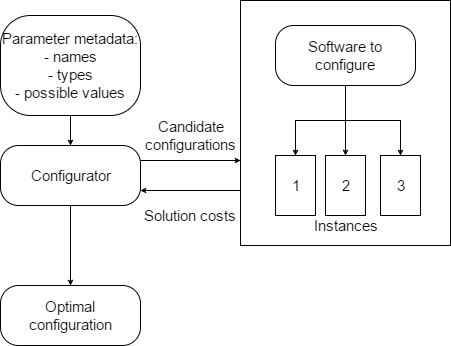
\includegraphics[scale=0.7]{configuration-top-level.png}
  \caption{Automatic configuration scheme}
  \label{fig:autoconf}
\end{figure}

Figure \ref{fig:autoconf} shows software composition of the analyzed program and configuration script. Configuration script has parameter metadata in its disposal. Based on them, the configuration software runs the software to configure with candidate configurations one by one according to the higher-mentioned racing algorithm. The result of the run is the solution cost of cumulative runs of the algorithm on the defined problem instances. After the racing process finishes, the configuration software renders the best configuration obtained. In the most general software case there are two measures of the performance - solution quality (to maximize) and computation time (to minimize).

There are two application modes:
\begin{itemize}
\item Offline tuning - introduces a learning stage on training instances before learning on the actual set.
\item Online tuning - tunes the parameters while solving the actual instance set.
\end{itemize}

A widely used configuration algorithmic family is racing algorithms. The simplified algorithm is shown in \ref{lst:racing} and an illustration is showed in \ref{fig:irace}.


\begin{minipage}[c, breaklines=true]{0.95\textwidth}
\begin{lstlisting}[caption={General racing pseudo-code}, label={lst:racing}]
procedure racing
start with an initial candidate set Theta
repeat iterations I
	process an instance stream
	evaluate the candidates sequentially
	remove inferior candidates
until winner is selected or exit condition fulfilled
end
\end{lstlisting}
\end{minipage}

\begin{figure}[H]
  \centering
    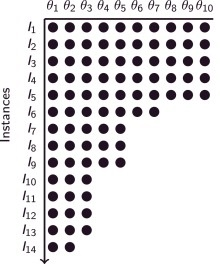
\includegraphics[scale=1.2]{irace.jpg}
  \caption{I-RACE execution illustration}
  \label{fig:irace}
\end{figure}


I-RACE(iterated race) implementation has already been developed and applied for the ACO problem in \cite{iraceaac}. It was implemented in R with taking into account the parallel programming techniques and initial candidate set-up. The feature of the IRACE is based on iterated generation of new configurations and removing of solutions with less fitness for further evaluating on the problem instances.


Two conceptual approaches can be remarked (although their distinction is ambiguous in particular cases):
\begin{itemize}
\item Top-down - develop a fixed template-based algorithm. It is based on strictly structured algorithm which allows some parametric configuration of some of its details with minor behavior modifications.
\item Bottom-up - algorithm is build of flexible components with some rule restrictions. Often involves application of genetic programming and evolution ideas.
\end{itemize}

\section{Research state}

The higher-mentioned ACOTSP framework accompanied by IRACE R script have already produced results for the TSP and the QAP problems. The results are described in the following two subsections. General conclusion during this research is that solutions obtained by the optimal configurations are better than those obtained by the default configurations. The comparison was carried out by measuring the deviation from the optimal solution for each instance.

\subsection{Finding a better ACO configuration for the TSP}

The optimal configuration is mentioned in the table \ref{table:table-tsp}, where it was computed for different algorithms. Various instances of different sizes were generated for the configuration process.

\begin{table}[ht]
\centering
\resizebox{\textwidth}{!}
{
\begin{tabular}{|r|r|r|r|r|r|r|r|r|r|r|r|r|}
  \hline 
    algo & $m$ & $\alpha$ & $\beta$ & $\rho$ & $q_0$ & $\epsilon$ & $cl$ & $nnls$ & $ph-limits$ & $slen$ & $restart$ & $res_{it}$\\ \hline
    ACS & 28 & 3.07 & 5.09 & 0.32 & 0.53 & 0.21 & 22 & 9 & - & - & branch-factor ($res_{bf} = 1.74$) & 212\\ \hline
	MMAS & 40 & 0.94 & 4.11 & 0.72 & 0.14 & - & 18 & 12 & yes & 191 & branch-factor ($res_{bf} = 1.91$) & 367\\ \hline
\end{tabular}
}
\caption{Optimal configuration for the TSP problem.}
\label{table:table-tsp} 
\end{table} 

With local search as 3-opt + dlb-bits.

\subsection{Finding a better ACO configuration for the QAP}

Problem instances were implemented in two forms - as RR or RS. In RR the distance matrix is computed as paired euclidean distances of points distributed on a square of length 300 in uniform way. The flow matrix is generated as a matrix of uniform random values within certain range. The RS distance matrix is generated in the same way, but the flow matrix adheres to real-world flow values.

100 instances were considered where half of them was used for training and the another half for testing. The best found configuration are shown in the table \ref{table:table-qap}.

\begin{table}[ht]
\centering
\resizebox{\textwidth}{!}
{
\begin{tabular}{|r|r|r|r|r|r|r|r|r|r|r|r|}
  \hline 
    & algo & $m$ & $\alpha$ & $\rho$ & $q_0$ & $dlb-bits$ & $ph-limits$ & $slen$ & $restart$ & $res_{it}$\\ \hline
    RR & MMAS & 6 & 0.324 & 0.29 & 0.062 & yes & no & 153 & distance ($res_{bf} = 0.051$) & 22\\ \hline
	RS & MMAS & 4 & 0.164 & 0.342 & 0.284 & yes & no & 170 & branch-factor ($res_{bf} = 1.822$) & 40\\ \hline
\end{tabular}
}
\caption{Optimal configuration for the TSP problem.}
\label{table:table-qap} 
\end{table} 

With local search as 2-best-opt.

\section{Conclusions}

Vast research work has been already conducted in terms of ACO algorithms. Many types of ACO algorithms and their extensions were developed and tested. However there are still many COPs untouched. In addition, various technical details can be added in order to improve resolution performance or the development experience. 

Various ways of further area research can be proposed. The possible way is to implement new NP-hard problems resolution algorithms within ACO framework. Such practical problems as Vehicle Routning Problem, Subset Sum Problem or Knapsack Problem.

From technical point of view we can propose implementing a new framework using object-oriented paradigm which will ensure high modularity and modification-proneness. Another option is to implement the ACO algorithm stages as parallel algorithms (stages like solution generation or local search).



\begin{thebibliography}{1}


\bibitem{aco_overview} Manuel L{\'o}pez-Ib{\'a}{\~n}ez and Thomas St{\"u}tzle {\em Ant Colony Optimization: A Component-Wise Overview} 2015: IRIDIA - Technical Report Series.

\bibitem{comb_opt} Papadimitriou CH, Steiglitz K {\em Ant Colony Optimization: A Component-Wise Overview} 1982: IRIDIA - Prentice Hall, Englewood Cliffs, NJ.

\bibitem{maniezzo} Maniezzo V {\em Exact and approximate nondeterministic tree-search procedures for the quadratic assignment problem} 1999: INFORMS Journal on Computing.

\bibitem{dorigo} Dorigo M, Gambardella LM {\em Ant Colony System: A cooperative learning
approach to the traveling salesman problem} 1997: IEEE Transactions on Evolutionary
Computation.

\bibitem{lookahead} Michel R, Middendorf M {\em An island model based Ant System with
lookahead for the shortest supersequence problem} 1998: Nature, PPSN V, Lecture Notes in Computer Science.

\bibitem{candidate_list} Dorigo M, Di Caro GA {\em The Ant Colony Optimization meta-heuristic} 1999: New Ideas in Optimization, McGraw Hill, London, UK.

\bibitem{hash_table} Alba E, Chicano F {\em ACOhg: dealing with huge graphs} 2007: Proceedings of the Genetic and Evolutionary Computation Conference.

\bibitem{iterated_greedy} Ruiz R, Thomas St{\"u}tzle {\em A simple and effective iterated greedy algorithm for the permutation flowshop scheduling problem} 2007: European Journal of Operational Research.

\bibitem{iterated_ants} Wolfram Wiesemann and Thomas St{\"u}tzle {\em Iterated Ants: An Experimental Study for the Quadratic Assignment Problem} 2006: Fachbereich Wirtschaftswissenschaften.

\bibitem{cunning_ants} Shigeyoshi Tsutsui {\em cAS: Ant Colony Optimization with Cunning
Ants} 2006: Hannan University, Matsubara Osaka.

\bibitem{mmas} Thomas St{\"u}tzle and Hoos HH {\em MAX–MIN Ant System} 2000: Future Generation Computer Systems.

\bibitem{ras} Bullnheimer B, Hartl R, Strauss C {\em A new rank-based version of the
Ant System} 1999: Central European Journal for Operations Research and Economics.

\bibitem{eas} Dorigo M {\em Optimization, learning and natural algorithms} 1992: Dipartimento di Elettronica, Politecnico di Milano, Italy.

\bibitem{bwas} Cordon O, de Viana IF, Herrera F, Moreno L {\em A new ACO model
integrating evolutionary computation concepts: The best-worst ant system} 2000: Second International Workshop on Ant Algorithms.

\bibitem{coop_tsp} Dorigo M, Gambardella LM {\em Ant Colony System: A cooperative learning
approach to the traveling salesman problem.} 1997: IEEE Transactions on Evolutionary
Computation.

\bibitem{iraceaac} Manuel L{\'o}pez-Ib{\'a}{\~n}ez  and  J{\'e}r{\'e}mie Dubois-Lacoste  and Leslie {P{\'e}rez C{\'a}ceres}  and  Thomas St{\"u}tzle  and  Mauro Birattari {\em Iterated Racing for Automatic Algorithm Configuration} 2013: IRIDIA - Technical Report Series.

\bibitem{aco_continuous} Socha K, Dorigo M {\em Iterated Racing for Automatic Algorithm Configuration} 2008: European Journal of Operational Research.
  
\bibitem{aco_incremental} Liao T, Montes de Oca MA, Aydin D, St{\"u}tzle T, Dorigo M {\em An incremental ant colony algorithm with local search for continuous optimization} 2011: Proceedings of the Genetic and Evolutionary
Computation Conference.  
  
\bibitem{moaco} L{\'o}pez-Ib{\'a}{\~n}ez M, St{\"u}tzle T {\em The automatic design of multi-objective ant colony optimization algorithms} 2012: IEEE Transactions on Evolutionary Computation.    
  
\bibitem{moba} Xin-She Yang {\em Bat Algorithm for Multi-objective Optimisation} 2011: Department of Engineering, University of Cambridge.  
 
 
\bibitem{external_memory} Dorigo, Marco
and Birattari, Mauro
and Blum, Christian
and Gambardella, Luca Maria
and Mondada, Francesco
and St{\"u}tzle, Thomas {\em IAn External Memory Implementation in Ant Colony Optimization} 2004: Springer Berlin Heidelberg - Proceedings.

\end{thebibliography}

 
\end{document} 
